\clearpage
\section{Satellite Formation Design}
\label{mtrSwarmDesign}
One of the most important aspects of this project is the fact that multiple satellites have to work in unison to achieve a common objective. This concept is called a constellation. In the case of Laser Swarm, it is necessary to design a formation as the platforms will need to be in close proximity to each other. 

A historical overview of satellite constellations presented on page 672 in \cite{constDesign} has yielded the fact that constellations are very mission specific and vary greatly. What is apparent though, is that altitudes of constellations are very high (1000 km and higher). This is mainly done in order to make stationkeeping easier as the main orbital perturbation, atmospheric drag, is less prominent.

In this section, the design of the swarm formation is looked at. Orbital characteristics are discussed in section \ref{mtrSwarmOrbitalParams}, while sections \ref{mtrSwarmStationkeeping} and \ref{mtrSwarmCollision} are concerned with stationkeeping and collision avoidance respectively. 
\subsection{Orbital Parameters}
\label{mtrSwarmOrbitalParams}

The relative motion of satellites flying in formation can be separated in 3 parts: large-scale relative motion due to satellites not being in the same orbit, small-scale motion due to individual perturbation effects and also the relative motion of one satellite as seen from the other.

The important thing to note is that for the design of the Laser Swarm, only a co-altitude constellation is considered. This will significantly simplify stationkeeping (all satellites have the same orbital period) as well as make instrument pointing much easier. Also two types of formation designs will be examined: along-track motion and cross-track motion. Along-track motion involves satellites following each other on the same orbit, while cross-track motion involves intersecting orbital planes at either same or varying orbit inclinations. 

The large-scale relative motion of two satellites in different orbits is governed by only two key variables: the relative inclination, $i_R$ and relative phase, $\phi_R$. The relative inclination is the angle at which the two orbit planes intersect. The relative phase is the angular separation of the satellites at the time they intersect each other's orbit plane. This happens four times per orbit. The two angles are shown in figure \ref{fig:relativeMotion} on page \pageref{fig:relativeMotion}.

\begin{figure}[ht!]
\centering
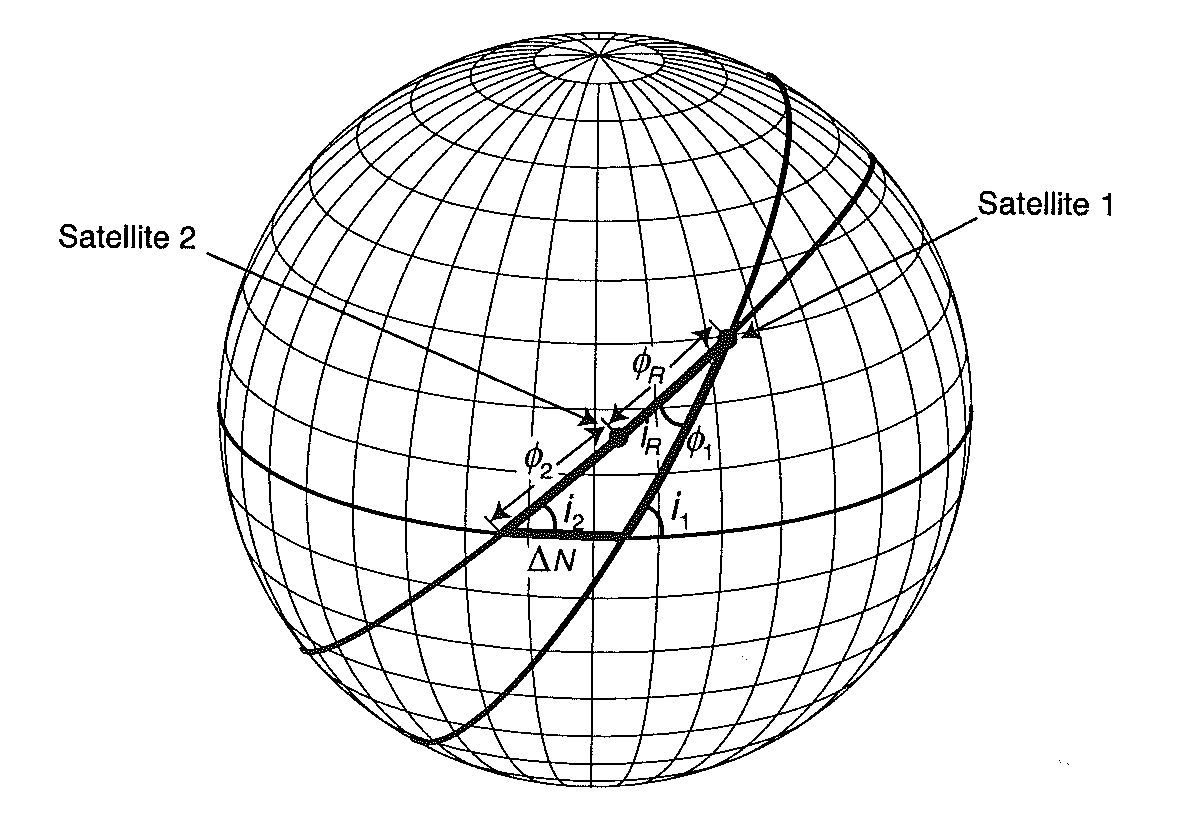
\includegraphics[width=0.75\textwidth, angle=0]{chapters/img/relativeMotion.png}
\caption{The relative motion of co-altitude satellites in circular orbits. Relative inclination and relative phase are shown. \emph{Source: \cite{constDesign}}}
\label{fig:relativeMotion}
\end{figure}

Two cases of cross-track motion exist: 

\begin{enumerate}
	\item Inclination of each orbital plane is the same ($i_1 = i_2 = i$) while the ascension nodes have a certain angular separation. This is the most common constellation type.
	\item Inclinations vary with each orbital plane. In this case all satellites can also have the same node of ascension, however this might not necessarily be the case.
\end{enumerate}

Out of the two cases, the most convenient one for the purpose of formation flying is method number 1. Since orbit precession is a function of only the inclination, it is smart to keep it the same for all satellites. This method is demonstrated in figure \ref{fig:intersection} on page \pageref{fig:intersection}.

\begin{figure}[ht!]
\centering
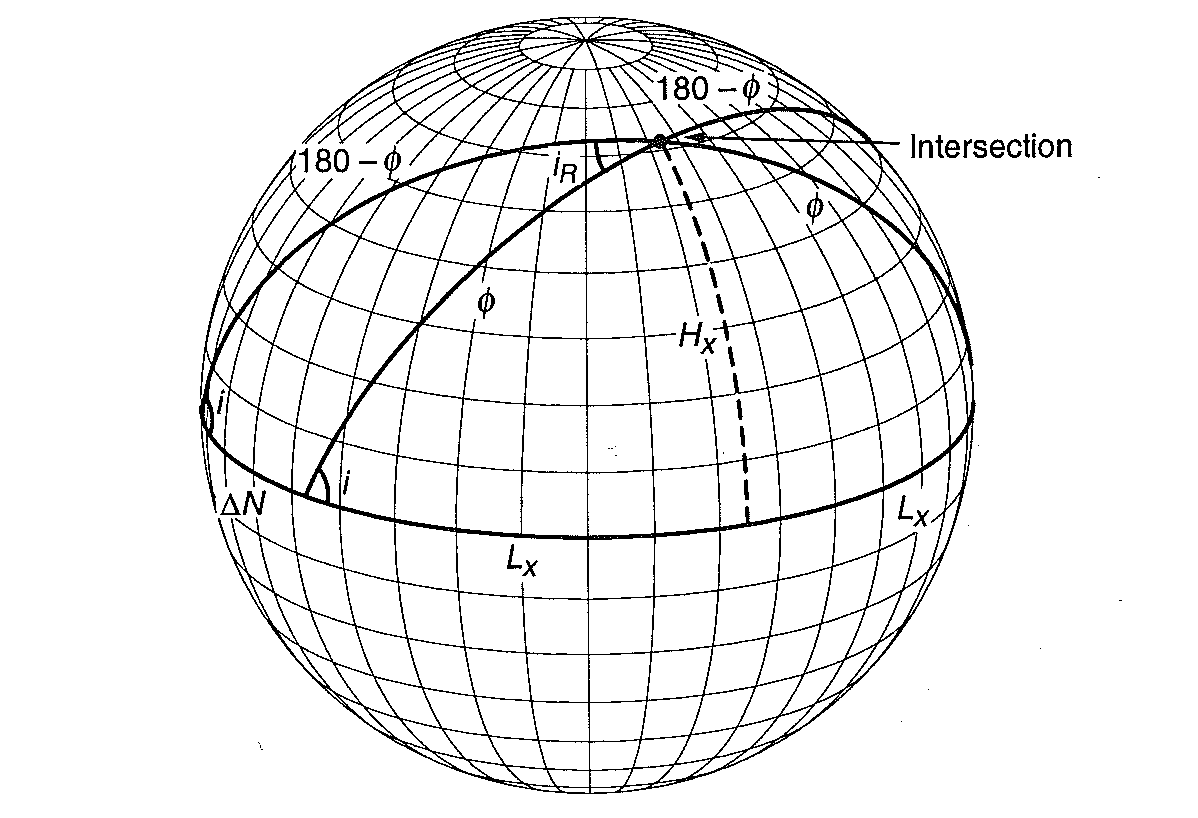
\includegraphics[width=0.75\textwidth, angle=0]{chapters/img/intersection.png}

\caption{Intersection of two orbits with the same inclination. \emph{Source: \cite{constDesign}}}
\label{fig:intersection}
\end{figure}

In figure \ref{fig:intersection} the $\Delta$N is the angular separation between the ascending nodes on the equator. For this case the following equations can be used:

\begin{equation}
cos i_R = cos^2i+sin^2i cos \Delta N
\label{ir}
\end{equation}
\begin{equation}
\phi_R = (T_2-T_1)n+ \Delta \phi
\label{phir}
\end{equation}
where
\begin{equation}
\Delta \phi = 180 - 2 \phi
\label{deltaPhi}
\end{equation}
\begin{equation}
tan \phi = \frac{tan ( 90 - \Delta N / 2)}{cos i}
\label{tanphi}
\end{equation}

Furthermore the relations for minimum and maximum angular separation of the two satellites are given:

\begin{equation}
sin ( \frac{\lambda_{min}}{2} ) = sin ( \frac{ \phi_R }{2} ) cos ( \frac{i_R}{2} )
\label{lambdamin}
\end{equation}

\begin{equation}
cos ( \frac{\lambda_{max}}{2} ) = cos ( \frac{ \phi_R }{2} ) cos ( \frac{i_R}{2} )
\label{lambdamax}
\end{equation}

The angular separation is a very important factor. To be able to determine the \ac{BRDF} of the surface under observation, the separation should be as large as possible, as the \ac{BRDF} is an angular property. However, for the purposes of \ac{ADCS} and inter-satellite communications, the separation should be kept small. Figure \ref{fig:earthangle} demonstrates the geometry of separation of the satellites.

\begin{figure}[ht!]
\centering
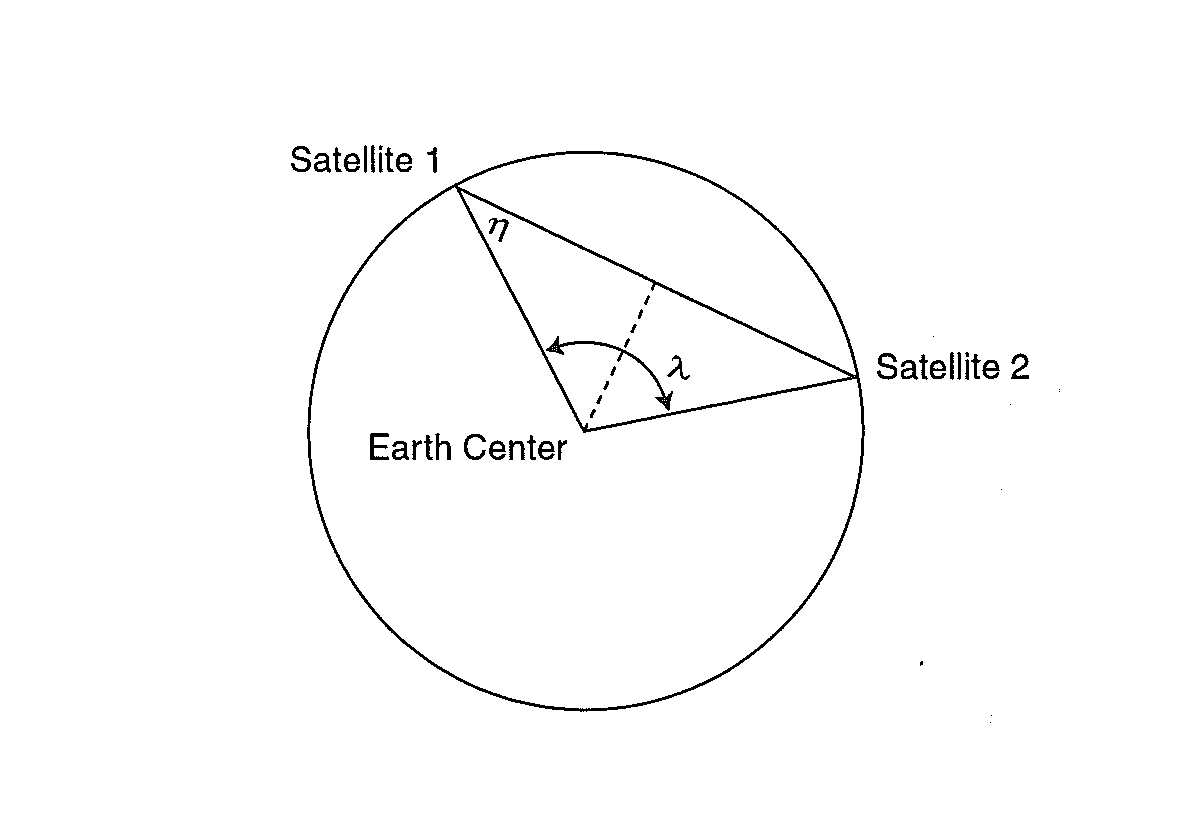
\includegraphics[width=0.75\textwidth, angle=0]{chapters/img/geometry.png}

\caption{Geometry of angular seperation. \emph{Source: \cite{constDesign}}}
\label{fig:earthangle}
\end{figure}

All of the above equations are in terms of degrees. Based on these relations it is possible to calculate the relationships between the equatorial angular separation and relative inclination, relative phase and the minimum and maximum angular separation.

\begin{figure}[ht!]
\centering
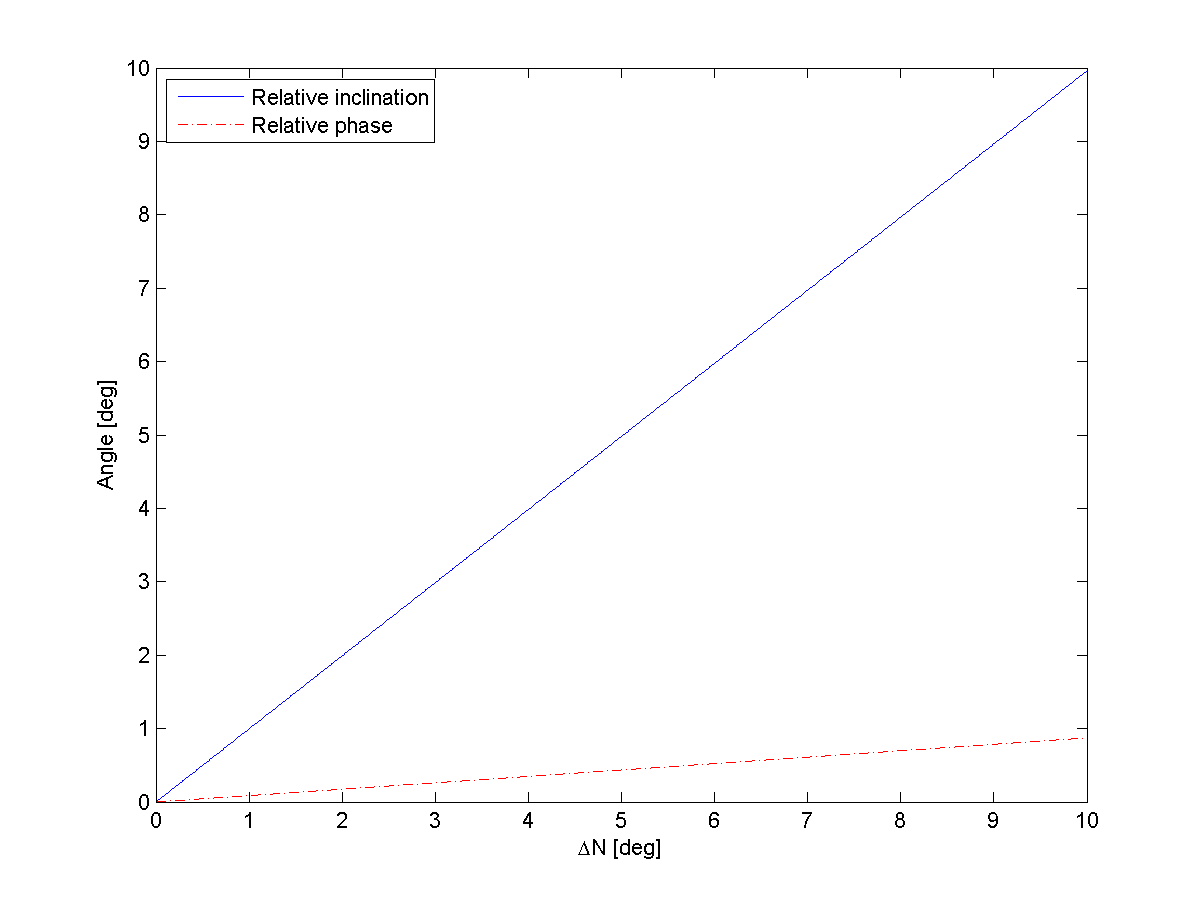
\includegraphics[width=0.75\textwidth, angle=0]{chapters/img/relativeInc.png}

\caption{$i_R$ and $\phi_R$ vs. equatorial angular separation. Orbit inclination of $85^o$.}
\label{fig:relativeI}
\end{figure}

\begin{figure}[ht!]
\centering
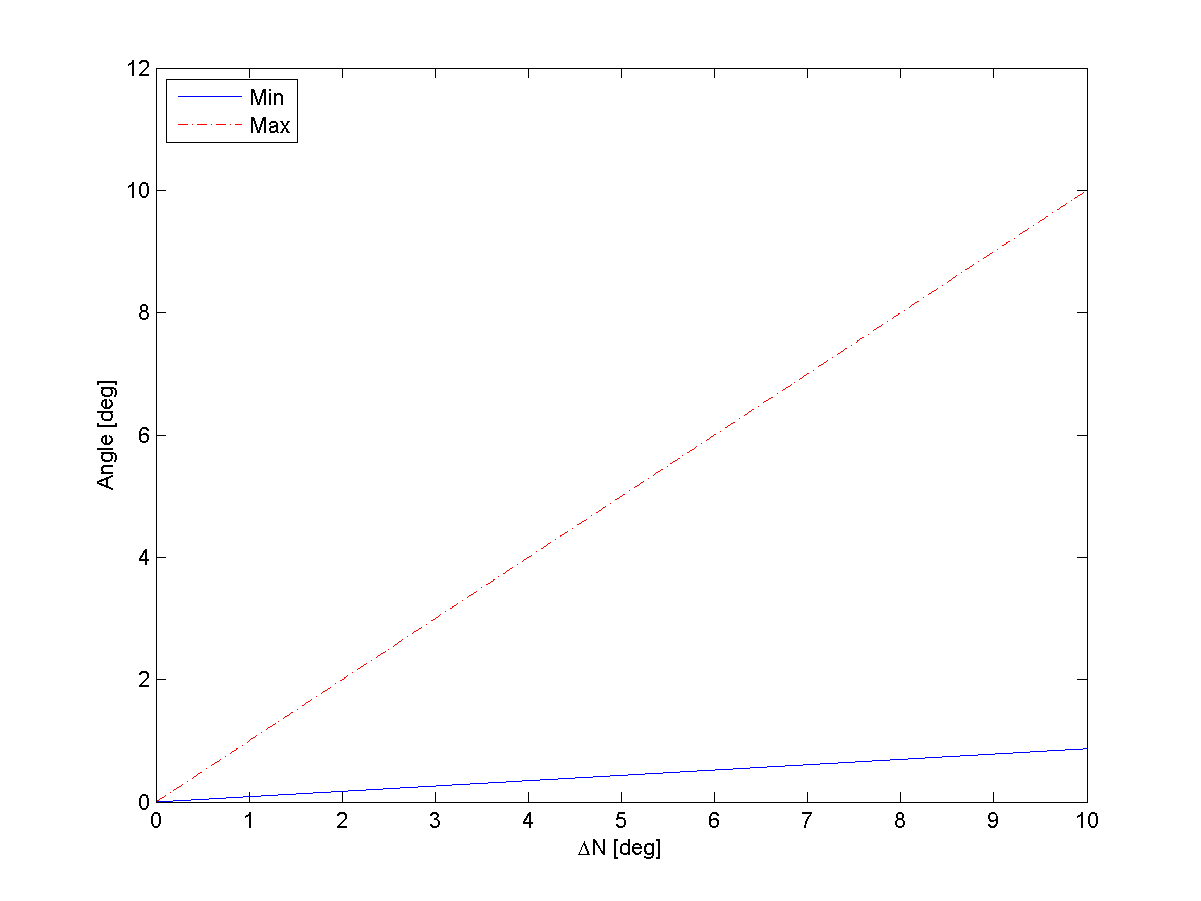
\includegraphics[width=0.75\textwidth, angle=0]{chapters/img/angularSeperation.png}
\caption{Minimum and maximum angular separation vs. equatorial angular separation. Orbit inclination of $85^o$.}
\label{fig:relativeSep}
\end{figure}

It is obvious from figures \ref{fig:relativeI} and \ref{fig:relativeSep} that the relative inclination and the maximum angular separation are almost equivalent to the equatorial separation. 

From the point of view of instrument pointing, the receiver should be at such separation from the emitter that the return signal is in the range of 1 to 30 degrees with respect to emitter nadir (for the outermost receiver satellite). This geometry is demonstrated in figure \ref{fig:separation}. This translates to a maximum angular separation of 2.18 degrees in both across-track and along-track directions. For along-track satellites that is simply a phase difference on the same orbit. For cross-track, the $\Delta N$ can be calculated to be 2.18 degrees as well. Resulting relative phase is 0.19 degrees. This is also then the minimum angular separation for the cross-track satellites.

The exact formation spread will be examined closer when the detail design will be performed, however it is assumed at this point that 2 satellites will be placed along-track (one fore and one aft of the receiver) and two satellites with across-track separation of 2.18 degrees. Depending on the results of the simulation concerning data processing, further satellites might be integrated into the swarm.

The relative analemma of two satellites in a 500 km orbit with a relative inclination of 2.18 degrees is shown in table \ref{table:analemma}.

\begin{table*}[ht]
	\centering
		\begin{tabular}{c |c | c }
		 \textbf{$i_R$} [deg] & \textbf{Across-track motion [deg]} & \textbf{Across-track motion [km]} \\ \hline \hline
		 2.18 & $\pm$ 2.18 & $\pm$ 262 
		\end{tabular}
	\caption{Height and width of the relative motion analemma for two co-altitude satellites in a 500 km orbit with an inclination of 85 degrees.}
	\label{table:analemma}
\end{table*}

\begin{figure}[!ht]
\centering
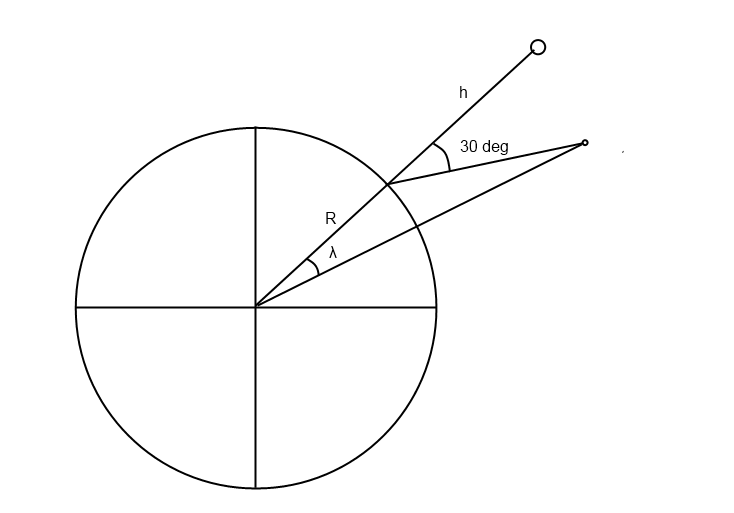
\includegraphics[width=0.75\textwidth, angle=0]{chapters/img/seperation.png}
\caption{Orbit separation geometry.}
\label{fig:separation}
\end{figure}

Small scale relative motion of the satellites will be looked at in more detail at later stages of the design.

\subsection{Stationkeeping}
\label{mtrSwarmStationkeeping}

Stationkeeping is the process of keeping the satellite within a well defined box relative to another satellite. The main reason for stationkeeping is overall maintenance of the constellation, and in the case of the Laser Swarm formation, for more accurate receiver pointing. When the receiver positions are well known and defined, maintaining concise data streams will be easier. Furthermore, precise stationkeeping reduces the chances of collisions and more precise inter-satellite communications.

Two main things that affect the relative positions of satellites:
\begin{itemize}
	\item Orbit perturbations such as atmospheric drag and Earth's oblateness effects, affect each satellite differently. One was of countering the complications concerned with drag were already discussed in section \ref{mtrAtmDrag}. It was noted that by keeping the ballistic coefficients of both the receiver and the emitter satellites as close together as possible, the orbit degradation due to drag will be similar for all satellites (since the formations are tight, it can be assumed that the air density experienced by all satellites is the same). This fact would entail that the same $\Delta$V impulse would be required for all platforms. Earth's oblateness effect constitutes the $J_2$ factor and causes the orbital precession. Over many orbits, the formation would drift apart if this effect was not managed. Since the rate of precession is a function of the semi-major axis, eccentricity and inclination, it is vital that these orbital parameters are kept constant for all satellites (as already noted in the previous section).
	\item Subtle variations in initial conditions can start a chain of events that will slowly drift the formation apart. Small variations in initial altitudes would mean small differences in orbital periods, and variations in inclination would give different rates of precession and would also increase risk of collision.
\end{itemize}

There are also three ways of dealing with perturbations for all satellites:

\begin{enumerate}
	\item Do nothing - do not compensate and let the formation float apart gradually. This option is not viable in the context of the mission lifetime. Orbits will completely decay before mission end.
	\item Control the perturbing disturbances to be the same for all satellites. In this case the satellites maintain the same relative position but cease to have Keplerian orbits. This option is also not viable as the payloads rely on precise orbits for pointing, and there is also no possibility to refocus the instruments.
	\item Negate the perturbing forces. All orbital characteristics are kept to the initial conditions by constant maintenance. Such perturbations as drag have to be constantly maintained in order to prevent the orbits from decaying. This is the only viable option in the context of the mission
\end{enumerate}

\begin{table}
	\centering
		\begin{tabular}{p{5cm}|p{5cm}|p{5cm}}
	\textbf{Perturbation} & \textbf{Impact} & \textbf{Handling} \\
		\hline \hline
		Atmospheric Drag & Secular decay ranging from 1-100 m/day & Altitude maintenance \\ \hline
		\multirow{4}{*}{Oblateness} & Secular node rotation of ~0.5 deg/day & Inclination maintenance \\ \cline{2-3}
		 & Secular phase rotation of 14 deg/day & Altitude maintenance \\ \cline{2-3}
		 & Changes in shape of orbit up to ~5 km variation between adjacent satellites & Uncompensated \\
    \hline
		\multirow{2}{*}{Solar/Lunar} & Secular drift in inclination and node of up to 3.5$*$10$^{-5}$ deg/day & Inclination maintenance\\ \cline{2-3}
		 & Low amplitude ascillations in inclination and node & Uncompensated \\ \hline
		Solar Radiation Pressure & Small & Typically uncompensated
	\end{tabular}
	\caption{Recommended methods of handling the principle perturbations in LEO. Source: \cite{constDesign}}
	\label{table:station}
\end{table}

Table \ref{table:station} on page \pageref{table:station} summarizes ways to handle perturbation stationkeeping. The concept can be implemented in two ways: relative and absolute stationkeeping. In the relative stationkeeping concept, the satellites are maintained in the same relative position to each other. In essence the situation may arise when the whole formation may be allowed to decay together. In contrast, absolute stationkeeping, maintains and controls each orbit separately. It has several advantages over the relative concept:

\begin{itemize}
	\item In practice, it has shown to use up less $\Delta$V.
	\item It is simple to command.
	\item Each satellite maintains itself in the pattern.
	\item Orbit position is precisely known without large data traffic.
	\item Can be fully autonomous.
	\item Easy monitoring from ground.
	\item Will not require instrument refocusing.
\end{itemize}
 
However it will require more constant attention. Absolute stationkeeping will be the right choice for the considered formation, as it will allow for greater accuracy of observation.    

\subsection{Collision Avoidance}
\label{mtrSwarmCollision}
Collision avoidance is an integral part of formation design, yet this analysis cannot be properly performed without the detail design of the constellation. However some design approximations can be already made to estimate the risks.

In the context of this formation, collision avoidance is important for two reasons: potential loss of two vehicles in a collision, one of them possibly being the emitter, and creation of a debris field which can jeopardize the safety of the rest of the platforms. A debris field evolution can be seen in figure \ref{fig:debris} on page \pageref{fig:debris}. 

\begin{figure}
  \centering
  \subfloat[]{\label{fig:elecMax}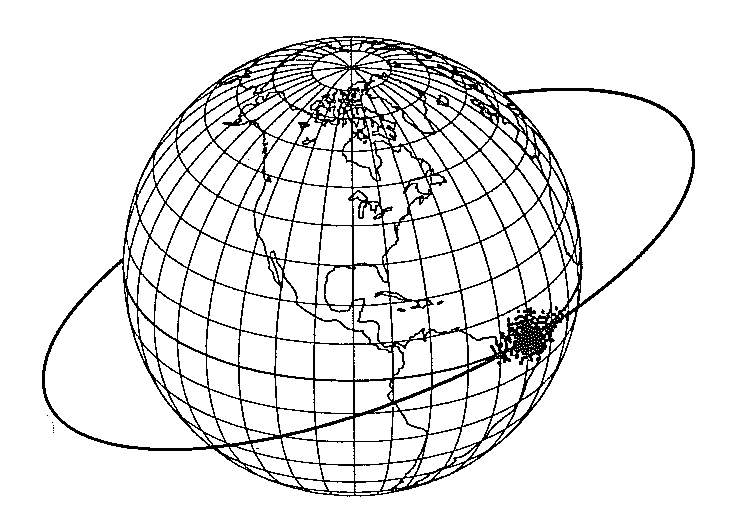
\includegraphics[width=0.5\textwidth]{chapters/img/collA.png}}                
  \subfloat[]{\label{fig:elecMin}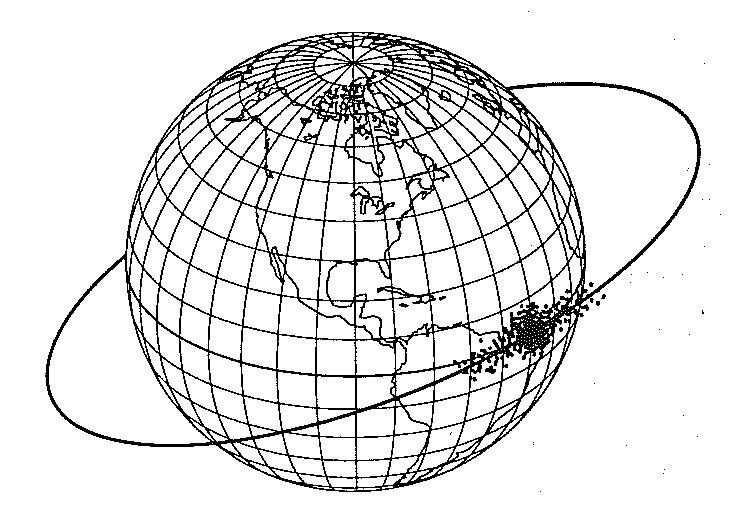
\includegraphics[width=0.5\textwidth]{chapters/img/collB.png}}\\
  \subfloat[]{\label{fig:elecMin}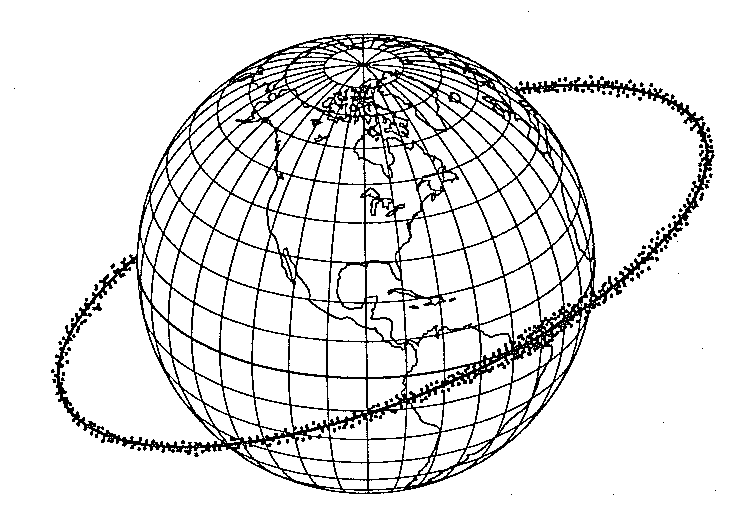
\includegraphics[width=0.5\textwidth]{chapters/img/collC.png}}
  \caption{Debris field evolution, (a) immediately after impact, (b) spreading out after some time and eventually settling into the orbit (c) and decaying. \emph{Source: \cite{constDesign}}}
  \label{fig:debris}
\end{figure}

Some prelimenary formation collision estimates are shown in table \ref{table:coll} on page \pageref{table:coll}. Based on this information it is obvious that the danger of a collision  between satellites rises exponentially as more platforms (and orbital planes) are introduced into the system.

\begin{table}
	\centering
	
		\begin{tabular}{p{5cm}|p{5cm}|p{5cm}}
	\textbf{Parameters} & \textbf{5 Satellite Formation in 3 Planes} & \textbf{9 Satellite Formation in 5 Planes} \\
		\hline \hline
		No. of satellites & 5 & 9 \\
		No. of orbit planes & 3 & 5 \\ 
		Vertical dispersion [km] & 1 & 1 \\
		In-track dispersion [km] & 276 & 276 \\
		Potential impact area [km$^2$] & 276 & 276 \\ 
		Collision opp. per orbit & 20 & 72 \\
		Orbit period [min] & 94.62 & 94.62 \\ 
		Collision opp. per year & 1.1$*$10$^5$ & 4.0$*$10$^5$ \\
		Collision opp. in 5 years & 5.6$*$10$^5$ & 2.0$*$10$^6$ \\
		Collision prob. per opp. & 1.0$*$10$^{-6}$ & 1.0$*$10$^{-6}$ \\
		Mean number of collisions per year & 0.11 & 0.4
		
			\end{tabular}
	\caption{Inter-satellite collision estimations for a formation of 5 and 9 satellites. Probability values based on extrapolation of values given in \cite{constDesign}.}
	\label{table:coll}
\end{table}

In order to successfully implement a safety-conscious formation design the following rules will have to be followed:
 
\begin{enumerate}
	\item Maximize spacing between platforms on orbit crossing.
	\item Remove satellites at end of life.
	\item Keep tracking the motion of "dead" satellites.
	\item Remove launcher upper stages from the orbits.
	\item Design replacement injections with collision avoidance in mind.
	\item Capture any ejected components.
	\item Avoid self-detonation.
\end{enumerate}
 
Following these rules will lead to a safer formation and eventually to an extended mission lifetime.

Another topic is collision avoidance of object that are outside the considered formation, however this discussion is out of the scope of this document and will be examined in further reports.